\graphicspath{{detail_design/fig/}}

\chapter{Detailed Design}
\label{chap:detail_design}

\begin{figure}[!h]
    \centering
    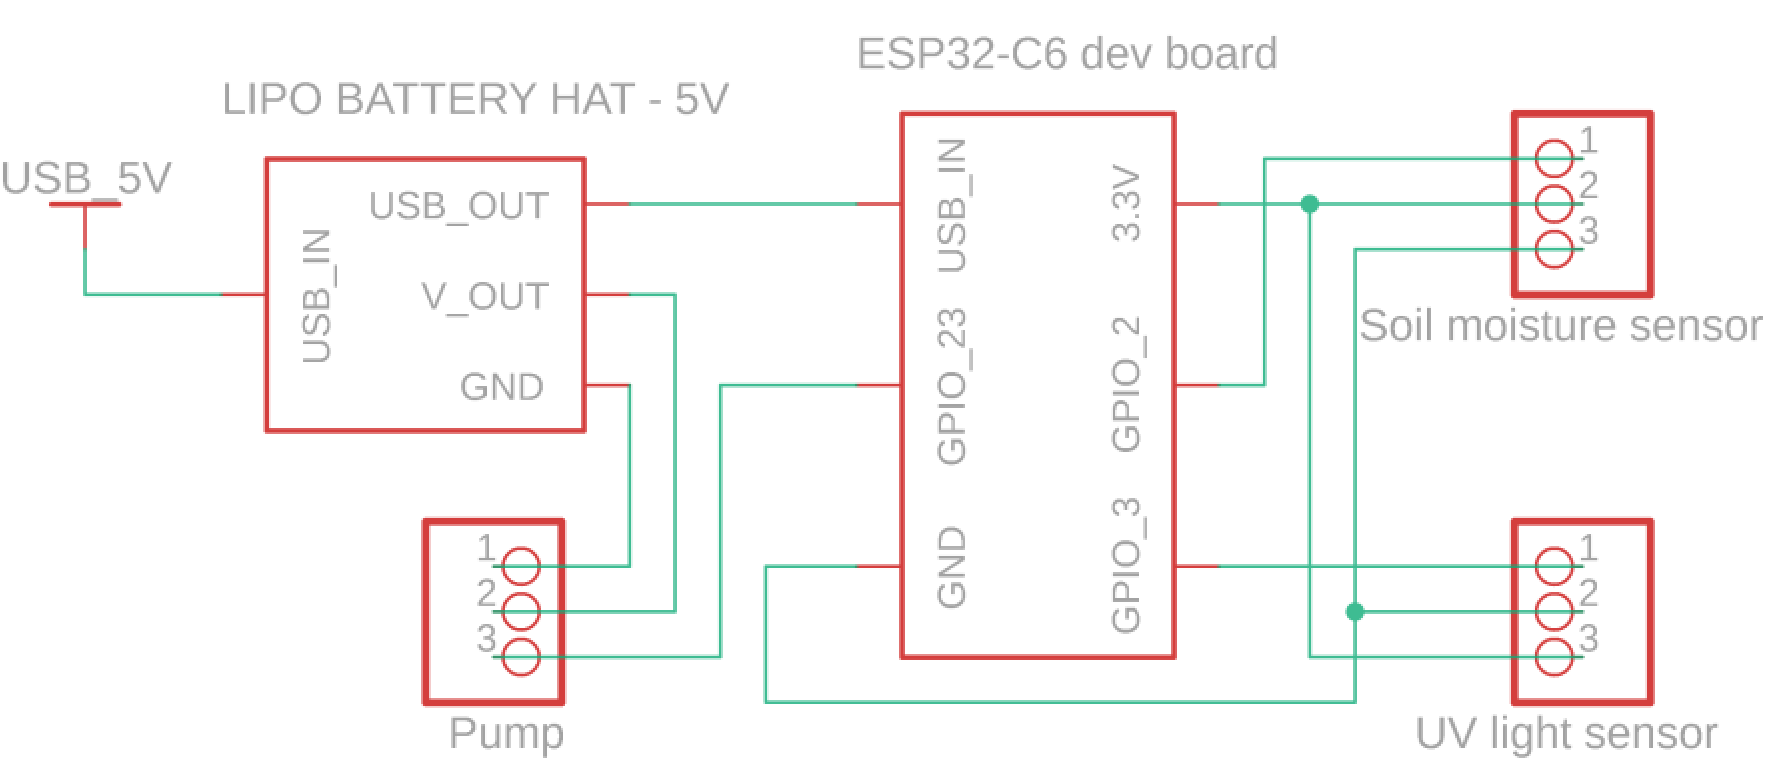
\includegraphics[width= 0.8\textwidth]{Report/detail_design/fig/detail_schematic.png}
    \caption{System schematic}
    \label{fig:detail_schematic}
\end{figure}

According to the electrical characteristics of the major components (shown in table \ref{tab:electrical_chars}), the entire system can be powered by a 5V source. The battery module will provide power to the pump and microcontroller. The sensors will be powered from the microcontroller 3.3V output. Pin 23 on the ESP32 is used to control the pump using a PWM signal, pins 2 and 3 receive the analog outputs from the soil moisture sensor and UV light sensor respectively. As shown in table \ref{tab:electrical_chars} the system will not exceed the battery module current capacity of 1.8A.

\begin{table}[!h]
\centering
\caption{Electrical characteristics of major components.}
\label{tab:electrical_chars}
    \begin{tabular}{|c||c|c||c|c|} 
        \hline
        Component & \multicolumn{2}{c||}{Input} & \multicolumn{2}{c|}{Output} \\
       %\hline
         & Voltage [V] & Current [mA] & Voltage [V] & Current [mA] \\
        \hline
        \hline
        ESP32 \cite{esp_datasheet} & 3.3 & 500 & & \\
         & 5 & & & \\
        \hline
        ESP32 pins \cite{esp_datasheet} & 0.75 * $V_{DD}$ & & 0.8 * $V_{DD}$ & 40\\
        & $V_{DD}$ + 0.3 & & & \\
        \hline
        Soil moisture sensor \cite{Moisture_sensor_datasheet} & 3.3 & $< 5$ \tablefootnote{Based off measurements} & 1.2 (high) & \\
        & 5.5 & & 2.5 (low) & \\
        \hline
        UV light sensor \cite{UV_sensor_datasheet} & 3 & 100 \tablefootnote{Maximum rating based off characteristics of similar sensors} & 0 & \\
        & 5 & & 3 & \\
        \hline
        Pump \cite{pump_datasheet} & 5 & 1000 & & \\
        \hline
        Battery module \cite{battery_datasheet} \cite{battery_faq} & 5  & 2500 & 5 & 1800 \\
        \hline
    \end{tabular}
\end{table}

%%%%%%%%%%%%%%%%%%%%%%%%%%%%%%%%%%%%%%%%
\section{Microcontroller}
Code for the microcontroller was written using the Arduino IDE, this was made possible by the esp32 (version 3.0.0-alpha3) board manager by Esspressif Systems and other contributors \cite{esp_arduino_github}. Data is stored using Firebase real-time and Firestore databases. Firebase was selected as it requires no additional device to act as a broker and allows the databases to be accessed remotely. It is also easily incorporated into Android apps using Android SDK. The Firebase Arduino client library for for Arduino devices by GitHub user mobizt (Suwatchai K.) and other contributors \cite{firebase_github} is used to interact with the databases.
\\

Three classes are used to manage external connections (Bluetooth and WiFi), data logging and uploading data. 
\begin{itemize}
    \item \textbf{DataLogger:} Calculates the average sensor readings.
    \item \textbf{ConnectionManager:} Manages the WiFi and Bluetooth connections.
    \item \textbf{DataManager:} Manages the connection to the Firebase databases, uploads logged data and retrieves device settings.
\end{itemize}

\begin{figure}[!h]
    \centering
    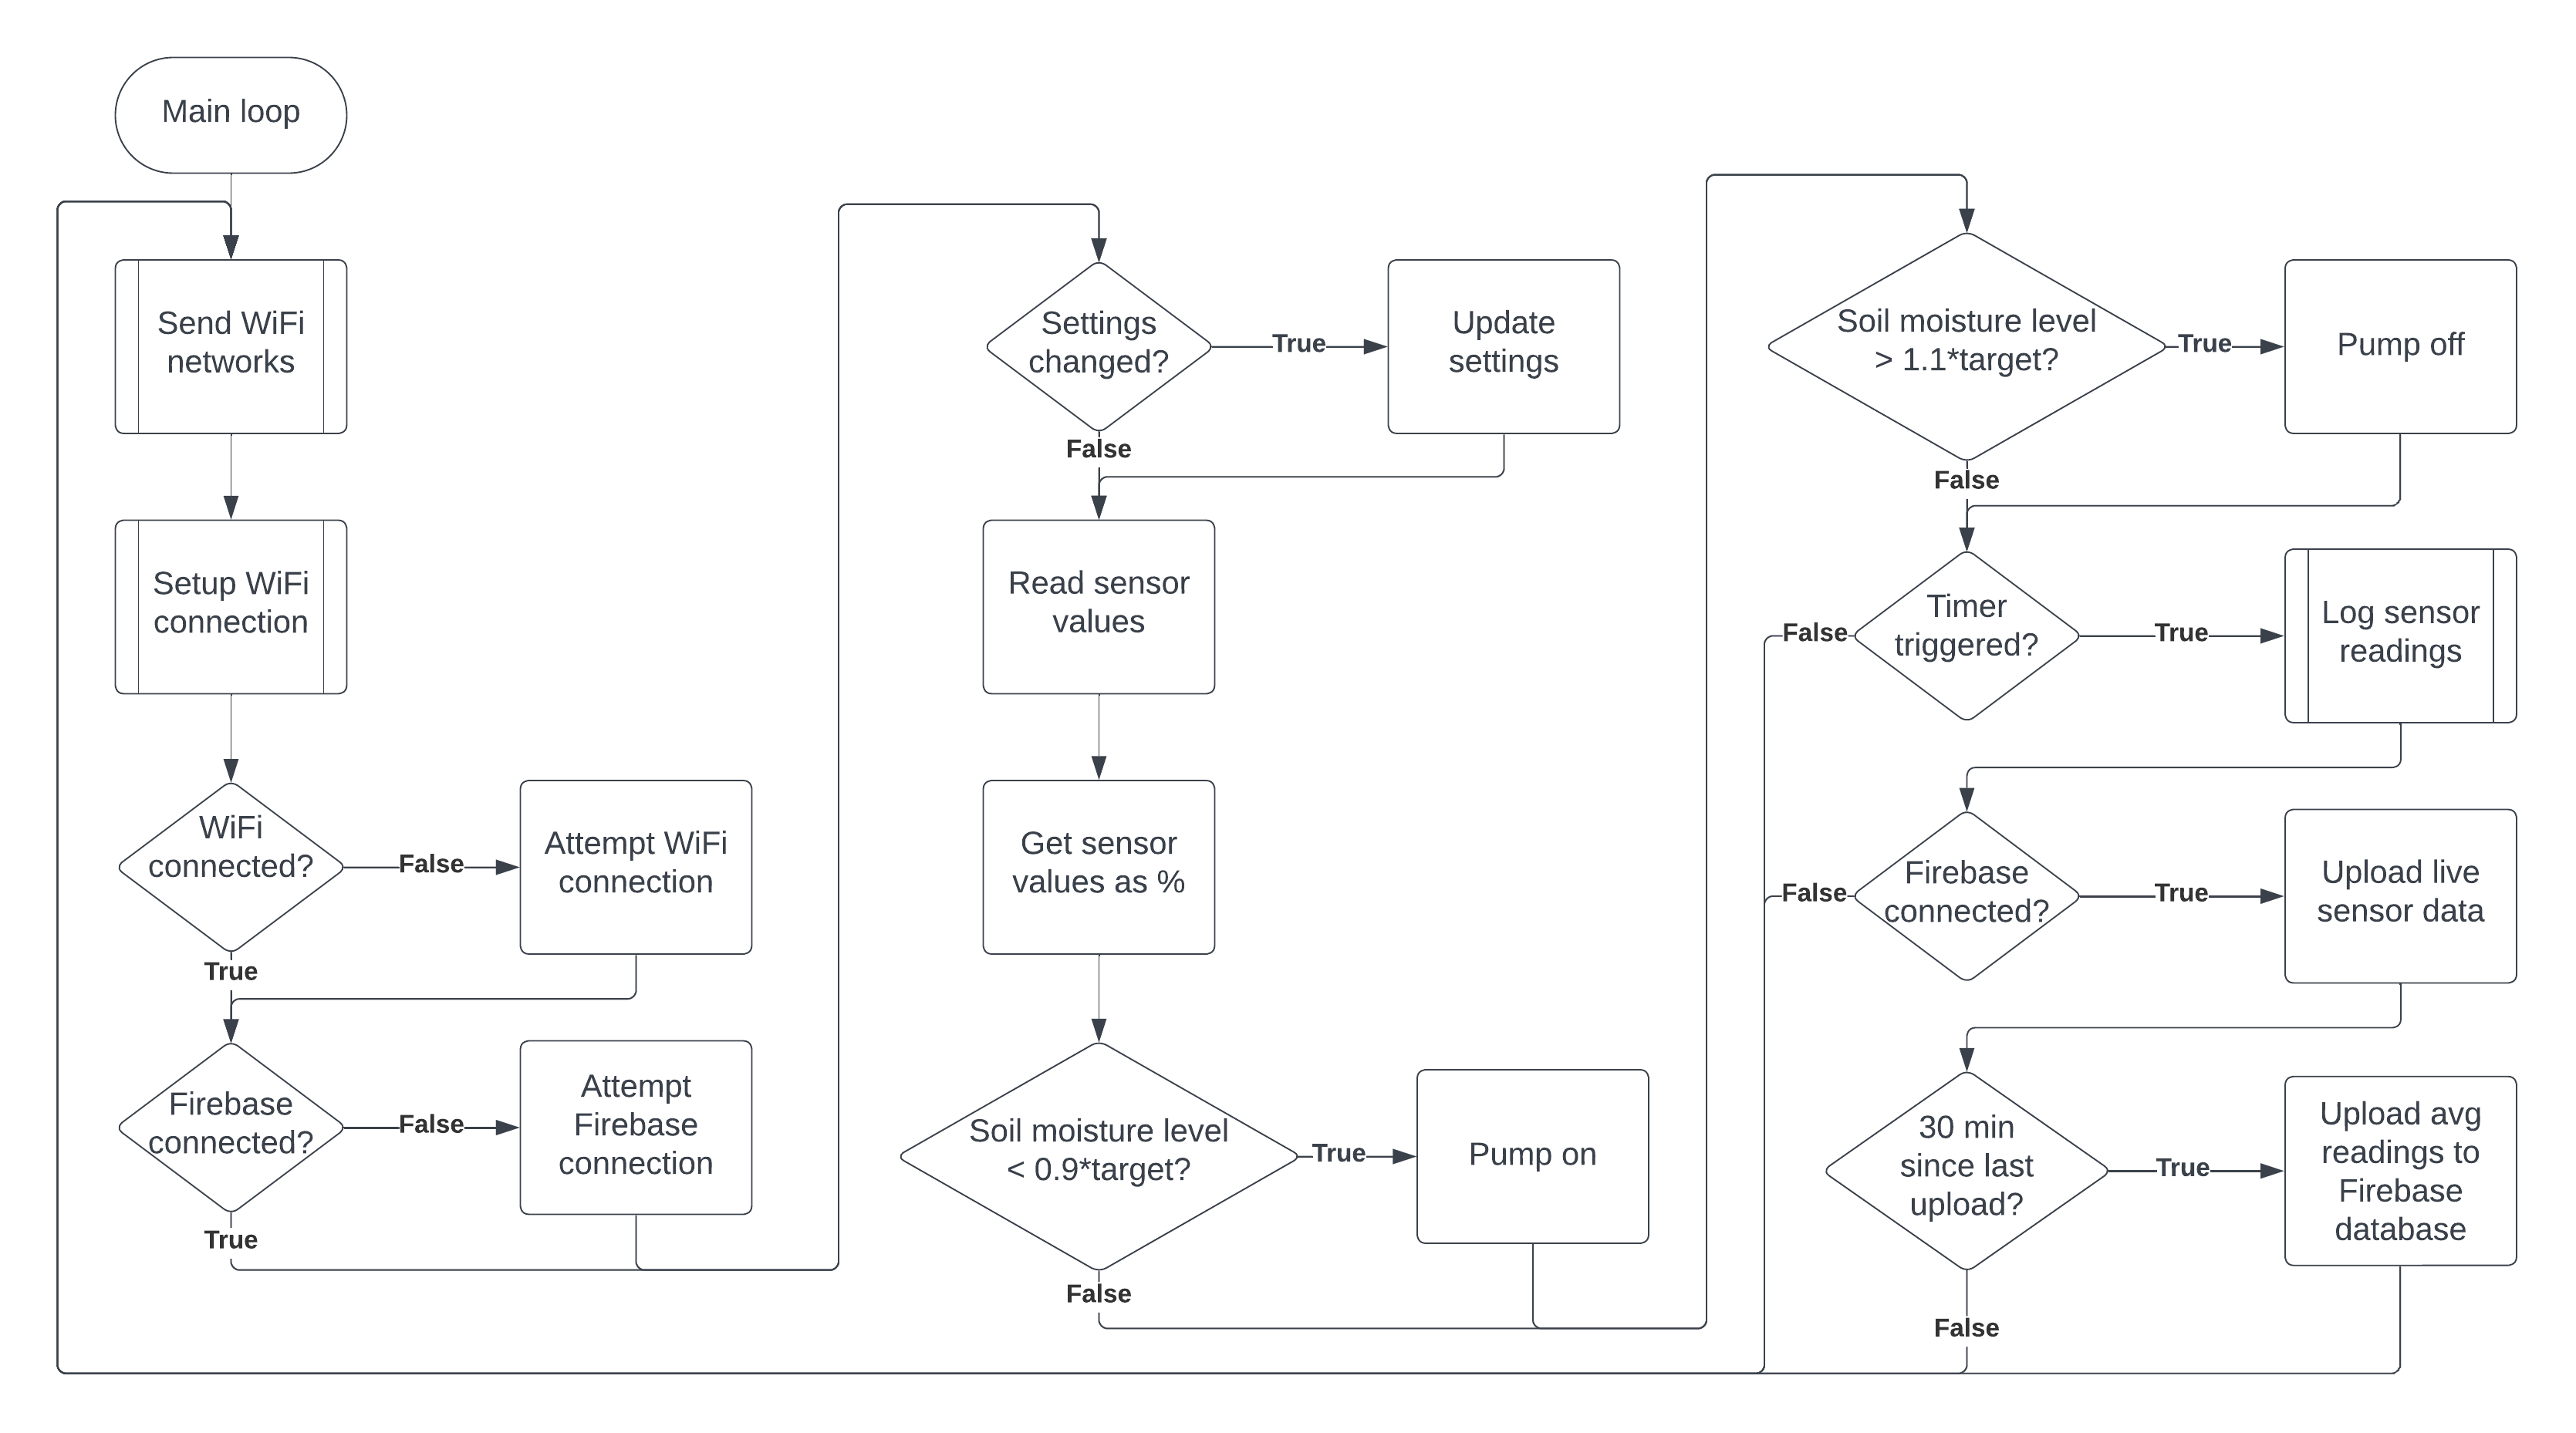
\includegraphics[width= 0.9\textwidth]{Report/detail_design/fig/main_loop_flow.png}
    \caption{Microcontroller code: main loop}
    \label{fig:main_loop_flow}
\end{figure}

The total sensor readings are updated in the main loop using a timer and interrupt that is triggered every minute. The current readings are also uploaded to the real-time database. Every 30 minutes the average sensor readings are calculated and uploaded to the Firestore database along with a timestamp.
\\
The current soil moisture levels are continuously compared to the target moisture level. The pump is turned on when the reading falls below $90\%$ of the target and is turned off once it reaches $110\%$ of the target level. Figure \ref{fig:main_loop_flow} shows a summary of the code described.

%%%%%%%%%%%%%%%%%%%%%%%%%%%%%%%%%%%%%%%%
\section{UV light exposure and soil moisture level measurement and logging}

The microcontroller uses a 5V supply to maximize the voltage output of the pins.
\\


Both the soil moisture and UV light sensors are designed to be powered by a microcontroller. Both sensors will therefore be powered using the 3.3V output pin on the ESP32. 
\\
Pins 2 and 3 (corresponding with ADC channels 2 and 3) will be used for the soil moisture and UV light sensor respectively

The default ADC measurement range of the ESP32-C6 is 0V to 1V \cite{esp_datasheet} \cite{esp_github}. The signals from the sensors must therefore be attenuated before being input to the ADC. The minimum attenuation as calculated in equation \ref{eqn:attenuation} \cite{attenuation_formula} is \(-10.37 dB\).

\begin{equation}
\label{eqn:attenuation}
\begin{split}
    Attenuation  (dB) & = 20 \cdot log_{10}\left ( \frac{V_{out}}{V_{in}} \right ) \\ 
    & = 20 \cdot log_{10}\left ( \frac{1}{3.3} \right ) \\ 
    & = -10.37 dB
\end{split}
\end{equation}

An attenuation of 11dB was used as it is the closest value provided by the ESP32 Arduino Core library \cite{esp_arduino_github} (which allows writing code for the ESP32-C6 using the Arduino IDE). 
\\
The ESP32-C6 has a 12 bit ADC \cite{esp_tech_ref}, resulting in a resolution of 4095, the sensor output ranges can be calculated using equation \ref{eqn:measured_val}. Table \ref{tab:sensor_ranges} shows the calculated measurement ranges of both sensors.

\begin{equation}
\label{eqn:measured_val}
    Measured \quad value = Resolution \cdot V_{in} \cdot 10^{Attenuation / 20}
\end{equation}

\begin{table}[!h]
    \centering
    \begin{tabular}{|c|cc|cc|}
    \hline
         & \multicolumn{2}{c||}{Soil moisture sensor} & \multicolumn{2}{c|}{UV light sensor} \\
        \hline
        Voltage & 1.2V & 2.5V & 0V & 3V \\
        Measured value & 1385 & 2885 & 0 & 3462\\
        \hline
    \end{tabular}
    \caption{Sensor value ranges}
    \label{tab:sensor_ranges}
\end{table}

%%%%%%%%%%%%%%%%%%%%%%%%%%%%%%%%%%%%%%%%
\section{Automatic watering}

%%%%%%%%%%%%%%%%%%%%%%%%%%%%%%%%%%%%%%%%
\section{App}

\begin{figure}[!h]
    \centering
    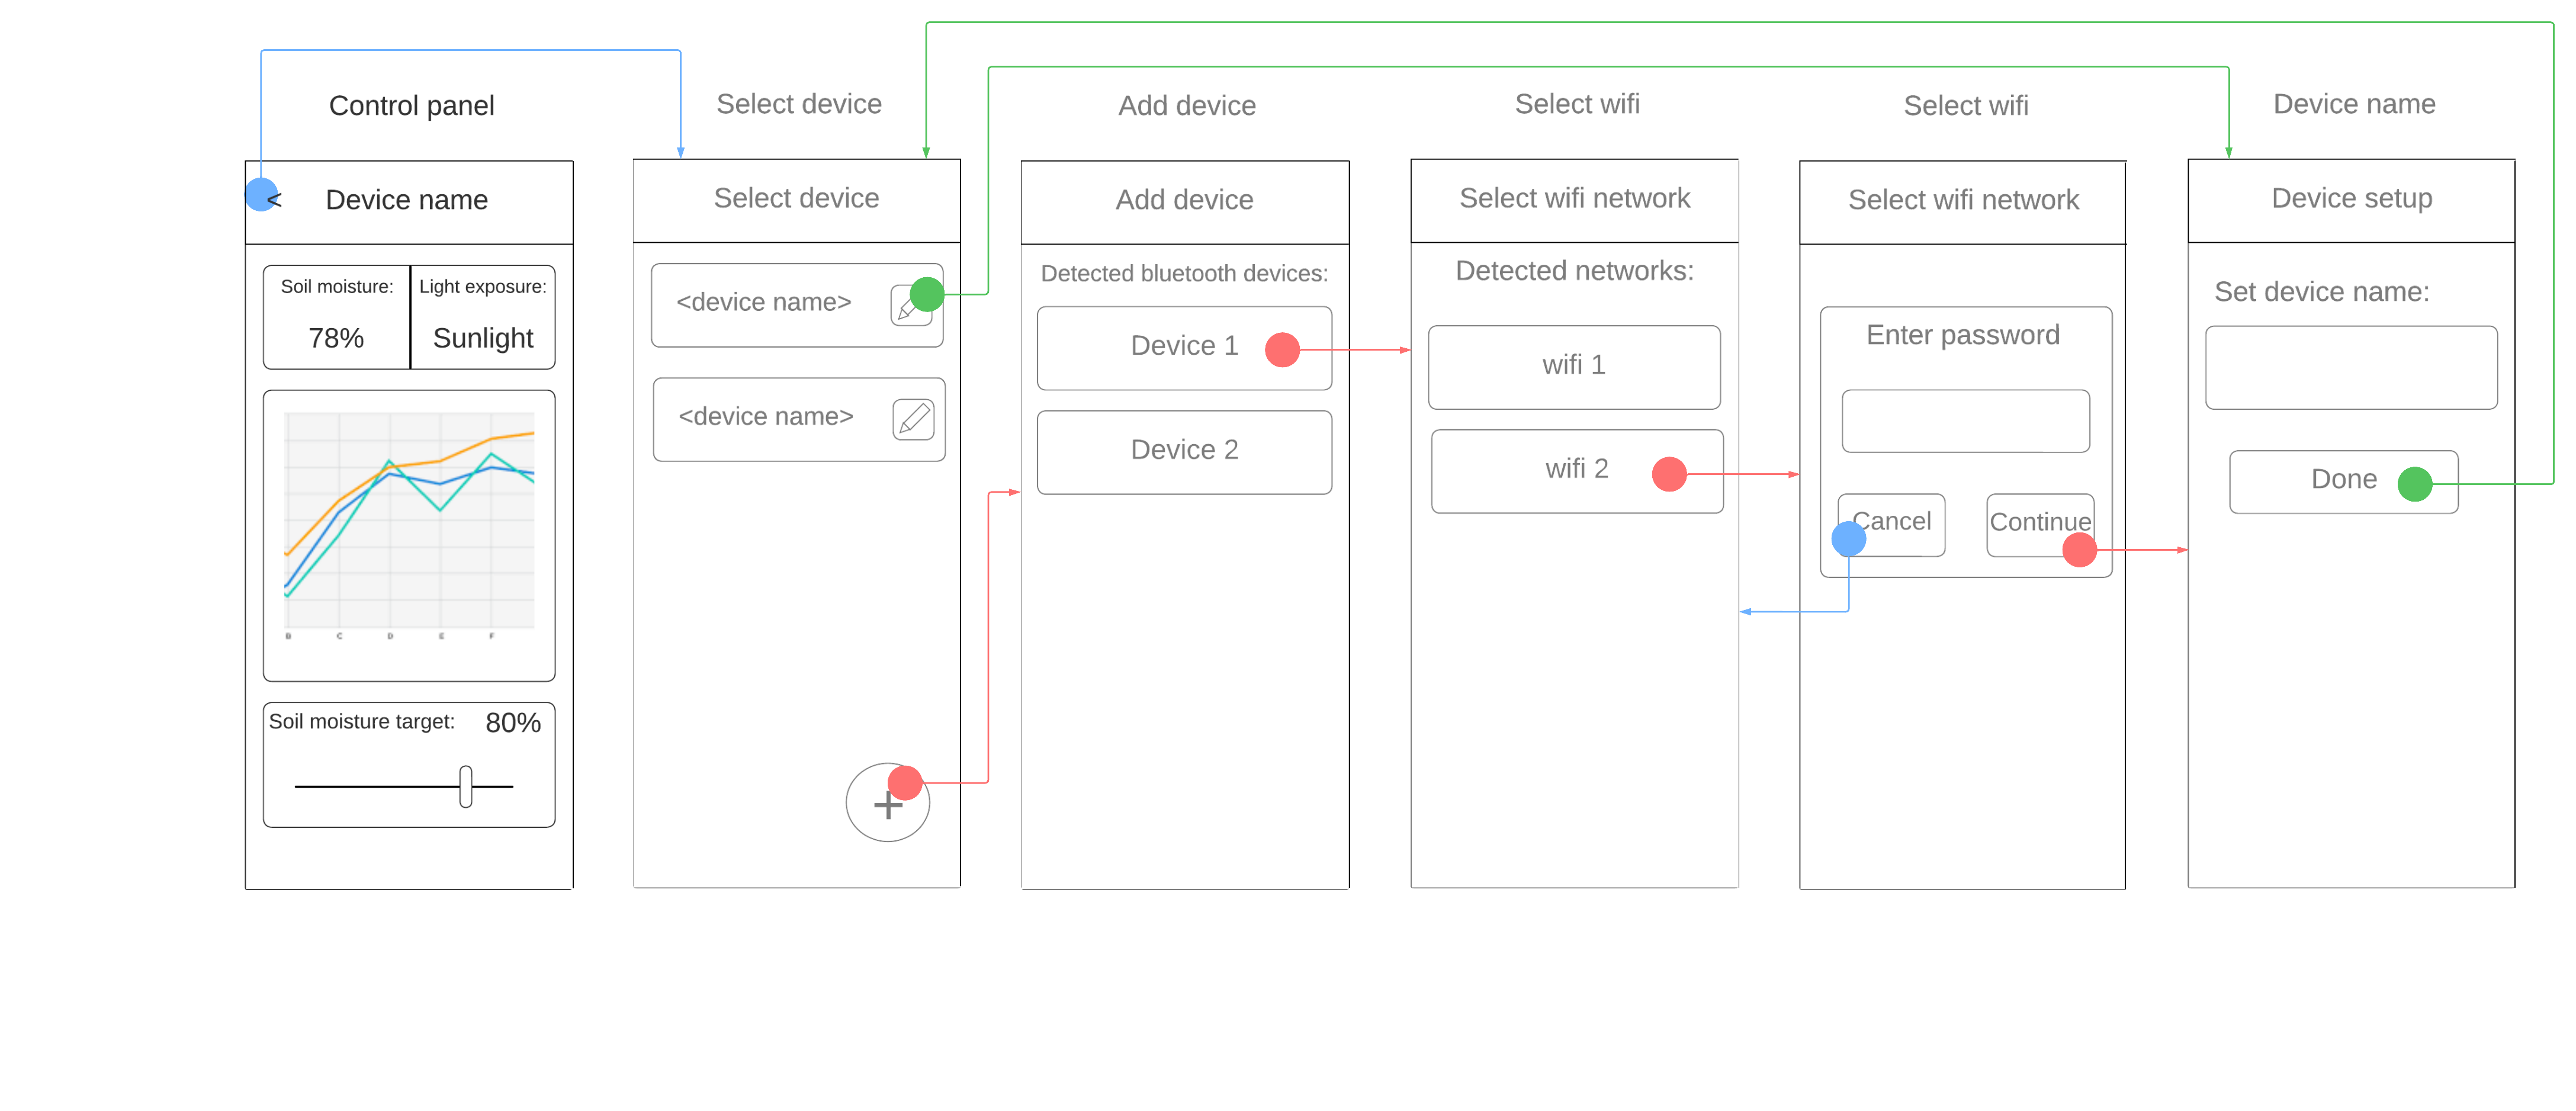
\includegraphics[width= \textwidth]{Report/detail_design/fig/app_flow.png}
    \caption{App flow}
    \label{fig:app_flow}
\end{figure}

\subsection{Connecting to WiFi}
\begin{figure}[!h]
    \centering
    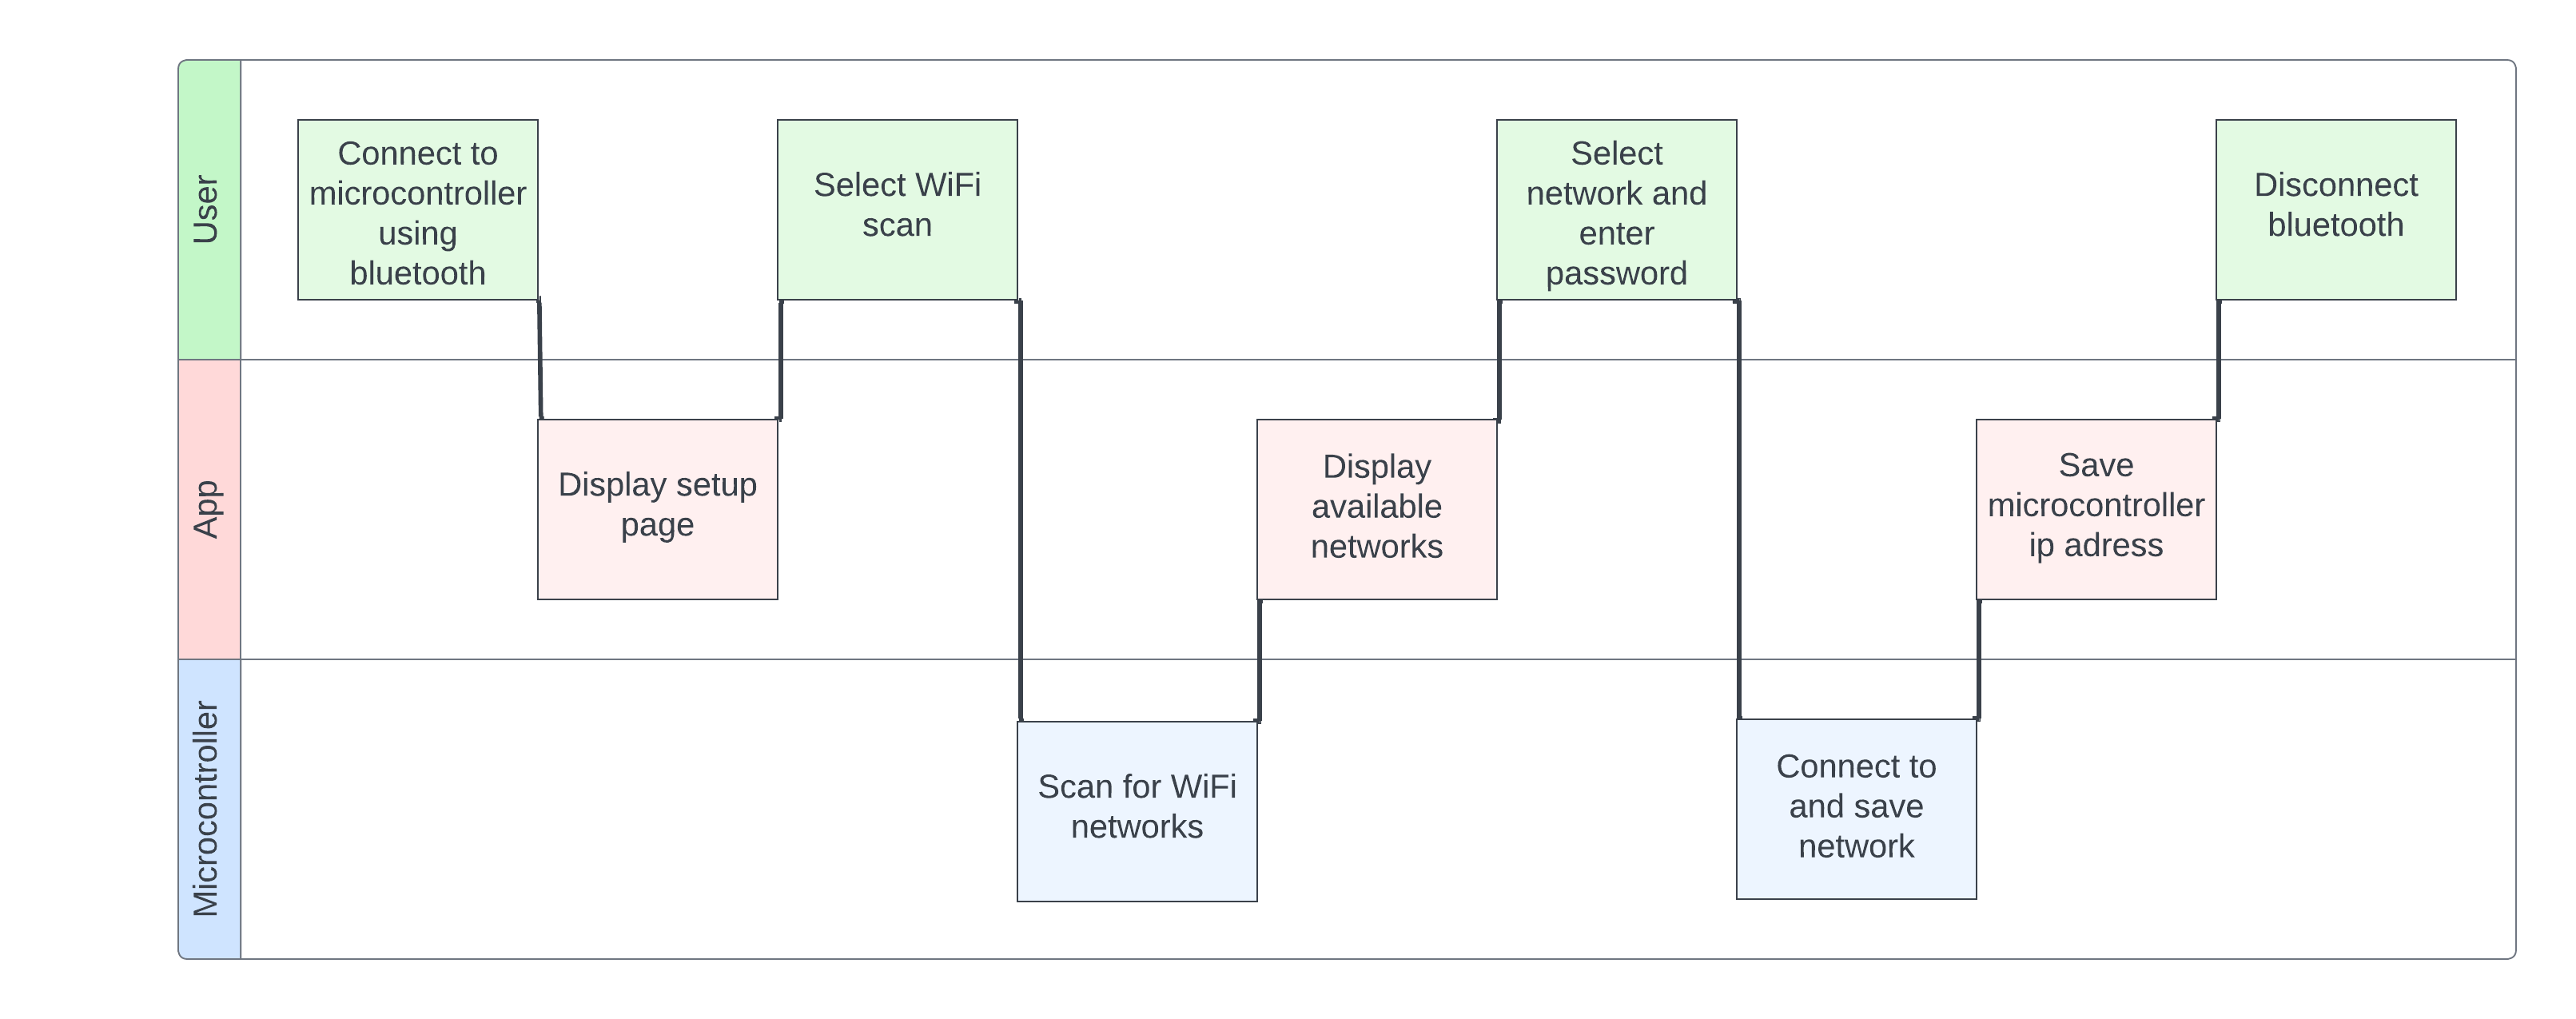
\includegraphics[width= \textwidth]{Report/detail_design/fig/wifi_connect.png}
    \caption{WiFi setup process}
    \label{fig:wifi_setup}
\end{figure}

%%%%%%%%%%%%%%%%%%%%%%%%%%%%%%%%%%%%%%%%
\section{Battery and charging}
\label{sec:battery}
\subsection{battery options}

%%%%%%%%%%%%%%%%%%%%%%%%%%%%%%%%%%%%%%%%
\section{PCB}

%%%%%%%%%%%%%%%%%%%%%%%%%%%%%%%%%%%%%%%%
\section{Case}
